\subsection{Example}\label{sec:example}
\newcommand{\pone}{$\langle service,owner=dataset.owner\rangle$}
\newcommand{\ptwo}{$\langle service,owner=partner(dataset.owner) \rangle$}
\newcommand{\pthree}{$\langle service, owner \neq dataset.owner AND owner \neq partner(dataset.owner)$}


In this section, we present an illustrative pipeline template, concentrating on the policy annotations.
The pipeline template consists of five stages, and each stage is noted with a policy.
All these policies are outlined in \cref{tab:anonymization}.
we recall that, \cref{tab:dataset} shows a sample of the dataset.
\hl{It is assumed that the Connecticut Prison (CTP) is the data owner, with partnerships with two other facilities, namely New York Prison and
  New Hampshire Prison.}\hl{SPOSTARE NEL SYSTEM MODEL?}

In the following we will make reference to three different type of anonymization:
\begin{enumerate*}[label=\roman*)]
  \item \emph{level0} (\tf{0}): no anonymization is performed;
  \item \emph{level1} (\tf{1}): the data is partially anonymized, only the first name and last name are anonymized;
  \item \emph{level2} (\tf{2}): the data is fully anonymized: first name, last name, identifier and age are anonymized.
\end{enumerate*}

Let us consider the pipeline template \tChartFunction in \cref{sec:example},
% 1° NODO %
The first stage consists of three parallel vertices (\vi{1}, \vi{2}, \vi{3}) and focuses on data collection without applying any policies.
The functional requirement necessitates a URI as input, and the output is the downloaded dataset.

The second stage incorporates a sole vertex, which merges the three datasets obtained from the previous stages and is associated with three policies (\p{1},\p{2},\p{3}).
The policies are evaluated during the node execution:
%if the service profile matches with the data owner ($owner = ``CTP"$), \p{1} is satisfied and the data is not anonymized (\tf{1});
%if the service profile matches with a partner of the owner ($owner = ``CTP"$), \p{2} is satisfied and the data is partially anonymized (\tf{2});
%if the service profile doesn't match with a partner nor with the owner ($owner = ``CTP"$), \p{3} is satisfied and the data is fully anonymized (\tf{3}).
% 2° NODO %
%he second vertex is responsible for enriching the data.
%The service downloads the dataset from partner facilities and enhances the dataset of the Connecticut facility.

if the service is by the data owner (\pone), which means that if the service owner is the same as the dataset owner, the owner dataset is not anonymized (\tf{0}).
if the service is by their partners (\ptwo), which means that if the service owner is a partner of the dataset owner, the dataset is level2 anonymized (\tf{1}).
if the service is by a third party  (\pthree), which means that if the service owner is neither the dataset owner nor a partner of the dataset owner, the dataset is level3 anonymized (\tf{2}).
The functional requirement necessitates $n$ datasets as input, and the output is the merged dataset.
% 3° NODO %
The third stage, is responsible both for data analysis/statistics and machine learning tasks.
The stage is composed of two alternative vertices respectively \vi{4}, \vi{5}.

Data analytics vertex adopts policies analogous to the second stage. The logic remains consistent:
if the service profile matches with the data owner (\pone), \p{1} is satisfied and the data computation is made level0 anonymized data (\tf{0});
if the service profile matches with a partner of the owner (\ptwo), \p{2} is satisfied and the data computation is made on level1 anonymized data (\tf{1});
if the service profile doesn't match with a partner nor with the owner (\pthree), \p{3} is satisfied and the data computation is made on level3 data (\tf{2}).
The functional requirement necessitates a dataset as input, and the output is the computes statistics.
% 4° NODO %
Machine Learning vertex adopts always a level3 anonymization (\p(4)) to prevent personal identifiers from entering into the machine learning algorithm/model (\tf{2}).
The functional requirement necessitates a dataset as input, and the output is the trained model or an inference.
% 5° NODO %
The fifth stage manages data storage.
If the service is within the facility itself ($\langle service,region=FACILITY"\rangle$), \p{5} is satisfied, resulting in data anonymization (\tf{1}).
Otherwise, if the service is in a partner region ($\langle service,region={CT,NY,NH}"\rangle$), the data undergo partial anonymization (\tf{2}).
The functional requirement necessitates some data as input, and the output is the URI of the stored data.
% 6° NODO %
The sixth stage is responsible for data visualization.
As stated in policy annotation \p{6}, if the user is member of the facility itself, the data are level0 anonymized (\tf{0}).
If the user is member of a partner facility, the data are  level2 anonymized (\tf{2}).
If the user is not member of the facility nor a partner, the data are level2 anonymized (\tf{3}).
The functional requirement necessitates a dataset as input, and the output is the visualization of the data.


In summary, this section has delineated a comprehensive pipeline template.
This illustrative pipeline serves as a blueprint, highlighting the role of policy implementation in safeguarding data protection across diverse operational stages.
\begin{table*}[ht!]
  \centering
  \caption{Anonymization policies}
  \label{tab:anonymization}
  \bgroup
  \def\arraystretch{1.5}

  \begin{tabular}[t]{c|c|l}
    \textbf{Vertex} & \textbf{Policy} & \policy{subject}{object}{action}{environment}{transformation}                                   \\ \hline

    \vi{M}          & $\p{1}$         & \policy{\pone}{dataset}{READ}{ANY}{ \tf{1}    }                                                 \\
    \vi{M}          & $\p{2}$         & \policy{\ptwo}{dataset}{READ}{ANY}{   \tf{2} }                                                  \\
    \vi{M}          & $\p{3}$         & \policy{\pthree}{dataset}{READ}{ANY}{    \tf{3}  }                                              \\
    \vi{4}          & $\p{4}$         & \policy{ANY}{dataset}{READ}{ANY}{    \tf{3}  }                                                  \\
    \vi{5}          & $\p{5}$         & \policy{$\langle service,region=``FACILITY"\rangle$}{dataset}{WRITE}{ANY}{ \tf{1}    }          \\
    \vi{5}          & $\p{6}$         & \policy{$\langle service,region=``\{CT,NY,NH\}"\rangle$}{dataset}{WRITE}{ANY}{   \tf{2} }       \\
    \vi{6}          & $\p{7}$         & \policy{$\langle user,role=   ``Connecticut Prison Officer"$}{dataset} {READ}{ANY}{ \tf{1}    } \\
    \vi{6}          & $\p{7}$         & \policy{$\langle user,role=   ``Partener Prison Officer"$}{dataset} {READ}{ANY}{   \tf{2} }     \\
    \vi{6}          & $\p{8}$         & \policy{$\langle user,role=   ``Any"$}{dataset} {READ}{ANY}{    \tf{3}  }                       \\
  \end{tabular}
  \begin{tabular}[t]{c|c|c}
    \textbf{\tf{i}} & \textbf{Level} & \textbf{Columns Anonymized}                  \\\hline
    \tf{0}          & Level0         & $anon(\varnothing)  $                        \\
    \tf{1}          & level1         & $anon(FIRST NAME, LAST NAME)$                \\
    \tf{2}          & level2         & $anon(FIRST NAME, LAST NAME, IDENTIFIER,AGE$ \\
  \end{tabular}

  %   % \begin{tabular}[t]{ccc}
  %   %   \toprule
  %   %   \textbf{Stage} & \textbf{Policy} & \textbf{Service} \\
  %   %   \midrule
  %   %   \vi{1}         & $p_1$           & $s_1$            \\
  %   %   \vi{1}         & $p_1$           & $s_2$            \\
  %   %   \vi{2}         & $p_2$           & $s_3$            \\
  %   %   \vi{2}         & $p_2$           & $s_4$            \\
  %   %   \vi{3}         & $p_3$           & $s_5$            \\
  %   %   \vi{3}         & $p_3$           & $s_6$            \\
  %   %   \bottomrule
  %   % \end{tabular}
  %   % \hspace{1em}

  %   \egroup
\end{table*}
\vspace{2em}

\begin{figure}[ht!]
  \centering
  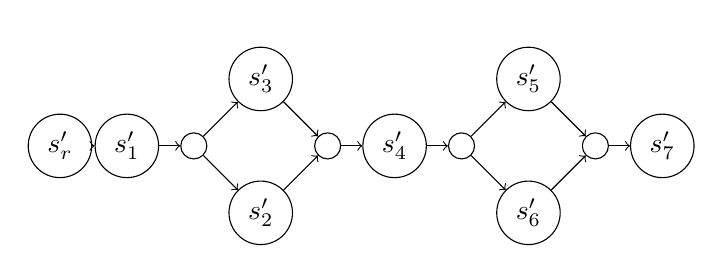
\begin{tikzpicture}[scale=0.85]
    \node[draw, circle] (node1) at (0,0) {$s^\prime_r$};
    \node[draw, circle] (node2) at (1,0) {$s^\prime_1$};
    \node[draw, circle] (node3) at (2,0) {$\timesOperator$};
    \node[draw, circle] (node4) at (3,-1) {$s^\prime_2$};
    \node[draw, circle] (node5) at (3,1) {$s^\prime_3$};
    \node[draw, circle] (node6) at (4,0) {$\timesOperator$};
    \node[draw, circle] (node65) at (5,0) {$s^\prime_4$};
    \node[draw, circle] (node7) at (6,0) {$\plusOperator$};
    \node[draw, circle] (node8) at (7,1) {$s^\prime_5$};
    \node[draw, circle] (node9) at (7,-1) {$s^\prime_6$};
    \node[draw, circle] (node10) at (8,0) {$\plusOperator$};
    \node[draw, circle] (node11) at (9,0) {$s^\prime_7$};
    % Text on top
    \node[above] at (node1.north) { \footnotesize$\instanceChartAnnotation$};
    \node[above] at (node2.north) { \footnotesize$\instanceChartAnnotation$};
    \node[above] at (node3.north) {};
    \node[above] at (node4.north) { \footnotesize$\instanceChartAnnotation$};
    \node[above] at (node5.north) { \footnotesize$\instanceChartAnnotation$};
    \node[above] at (node65.north) { \footnotesize$\instanceChartAnnotation$};
    \node[above] at (node8.north) { \footnotesize$\instanceChartAnnotation$};
    \node[above] at (node9.north) { \footnotesize$\instanceChartAnnotation$};
    \node[above] at (node11.north) { \footnotesize$\instanceChartAnnotation$};
    % Connection
    \draw[->] (node1) -- (node2);
    \draw[->] (node2) -- (node3);
    \draw[->] (node3) -- (node4);
    \draw[->] (node3) -- (node5);
    \draw[->] (node5) -- (node6);
    \draw[->] (node4) -- (node6);
    \draw[->] (node6) -- (node65);
    \draw[->] (node65) -- (node7);
    \draw[->] (node7) -- (node8);
    \draw[->] (node7) -- (node9);
    \draw[->] (node8) -- (node10);
    \draw[->] (node9) -- (node10);
    \draw[->] (node10) -- (node11);
  \end{tikzpicture}
  \caption{Service composition instance}
  \label{fig:service_composition_instance}
\end{figure}
